\section{Vakkarima vastagsága és karima szabványok}

\subsection{Minimális vastagság}
\begin{equation}
	d_t = \frac{(d_1 - 2s) + d_4}{2} = \siunit{\karimaDt}{\mm}
\end{equation}

\begin{align}
	&y_k = \frac{k}{\pi} \\
	&y_d = \frac{2}{3} \frac{d_t}{\pi} \\
\end{align}

\begin{equation}
	b_{\text{min}} 
	= \frac{d_t}{2} \sqrt{\frac{3p_\text{ü}}{\sigma_{\text{hajl}}} \left(1-\frac{2}{3} \frac{d_t}{k}\right)} 
	= \siunit{\karimabmin}{\mm}
\end{equation}

\begin{align}
	&\sigma = 
	\frac{d_{t}^2}{4} 
	\frac{3p_{\text{ü}}}{b_{\text{min}}^2}
	\left(1-\frac{2}{3}\frac{d_t}{K}\right) = \mpa{\karimasigma} \\
	&n = \frac{\sigma_{\text{hajl}}}{\sigma} = \siunit{\kariman}{-}
\end{align}

\newpage
\begin{figure}[hbt!]
	\centering
	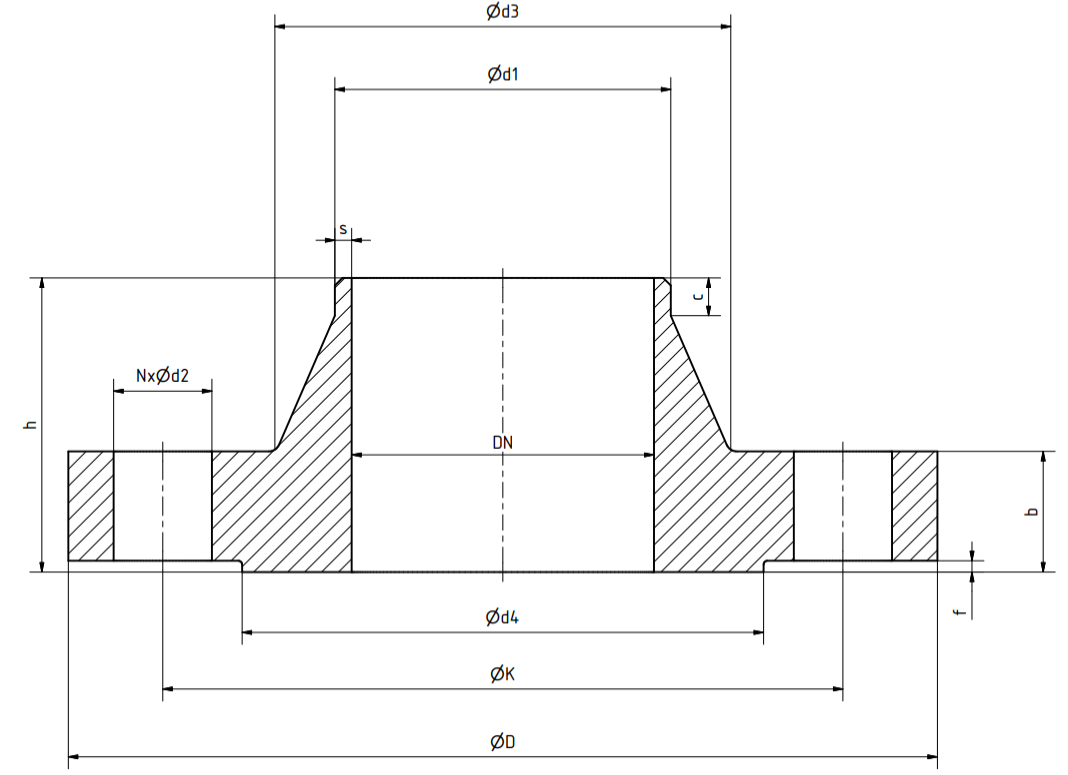
\includegraphics[scale=.61]{./images/karima.png}
	\caption{Karima előtervének rajza}
\end{figure}
\begin{align*}
	&D = \siunit{\karimaD}{\mm} \\
	&f = \siunit{\karimaf}{\mm} \\
	&d_4 = \siunit{\karimadfour}{\mm} \\
	&d_2 = \siunit{\karimadtwo}{\mm} \\
	&s = \siunit{\karimas}{\mm} \\
	&N = \siunit{\karimaN}{db} \\
	&K = \siunit{\karimaK}{\mm} \\
	&b = \siunit{\karimab}{\mm} \\
	&d_3 = \siunit{\karimadthree}{\mm} \\
	&d_1 = \siunit{\karimadone}{\mm} \\
	&M = \text{M24} \\
	&h = \siunit{\karimah}{\mm} \\
\end{align*}

\newpage
\begin{figure}[hbt!]
	\centering
	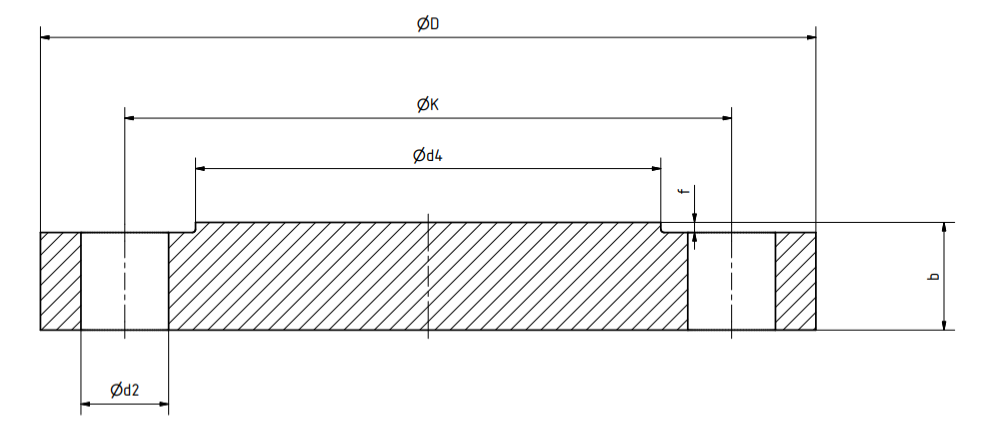
\includegraphics[scale=.34]{./images/vakkarima.png}
	\caption{Vakkarima előtervének rajza}
\end{figure}
\begin{align*}
	&D = \siunit{\karimaD}{\mm} \\
	&f = \siunit{\karimaf}{\mm} \\
	&d_4 = \siunit{\karimadfour}{\mm} \\
	&d_2 = \siunit{\karimadtwo}{\mm} \\
	&K = \siunit{\karimaK}{\mm} \\
	&b = \siunit{\karimab}{\mm} \\
\end{align*}
